\documentclass[11pt, a4paper]{article}

\usepackage[utf8]{inputenc}
\usepackage[greek, english]{babel}
\usepackage{alphabeta}
\usepackage{libertine}
\usepackage{graphicx}
\usepackage{biblatex}[sorting=nty] % sort alphabetically
\usepackage[table]{xcolor}
\usepackage{mathptmx} % Times New Roman
\usepackage{makecell}
\usepackage{setspace}
\usepackage{geometry}
\usepackage{booktabs}

\pagenumbering{arabic}
\onehalfspacing % Set line spacing to 1.5
\graphicspath{ {./output/} }
\addbibresource{refs.bib}

\def\code#1{\texttt{#1}}

\title{\Huge LLM Detection\\
	\LARGE Practical Data Science: 3rd Project}

\author{\Large  Tsirmpas Dimitris }


\begin{document}
	
	\maketitle
	\begin{center}
		\large Athens University of Economics and Business \\
		\large MSc in Data Science
		
	\end{center}
	
	
	\section{Introduction}
	This report outlines results and conclusions drawn from the LLM detection project which can be found at \url{https://github.com/dimits-exe/practical_data_science}. Implementation details, methodology and discussion can be found inside the relevant notebook and README file.
	
	
	
	\section{LLM Detection Results}
	
	Below we present graphs resulting from the LLM detection models presented in the original notebook.
	
	\begin{figure}
		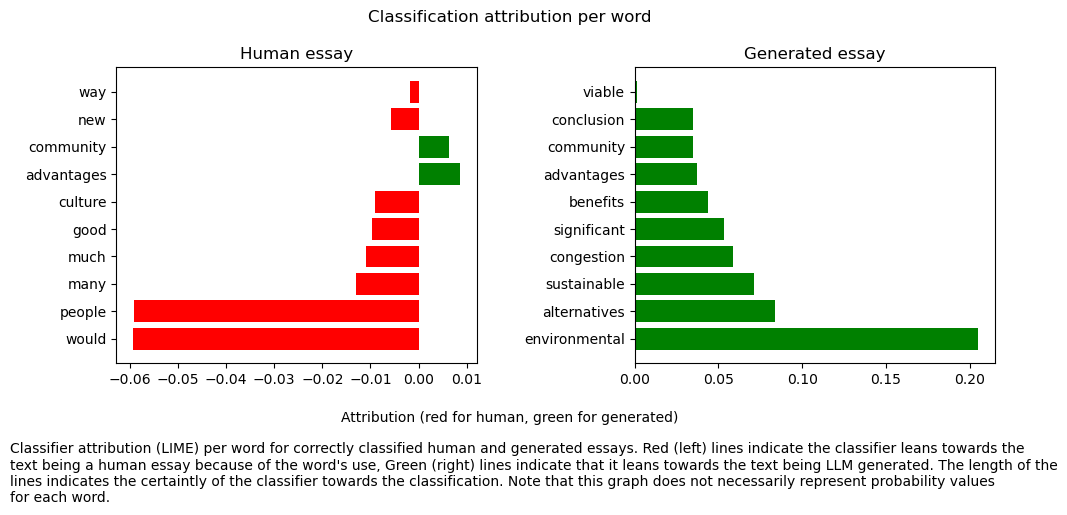
\includegraphics[width=14cm]{attribution.png}
		\centering
		\label{fig::attribution}
	\end{figure}
	
	\begin{figure}
		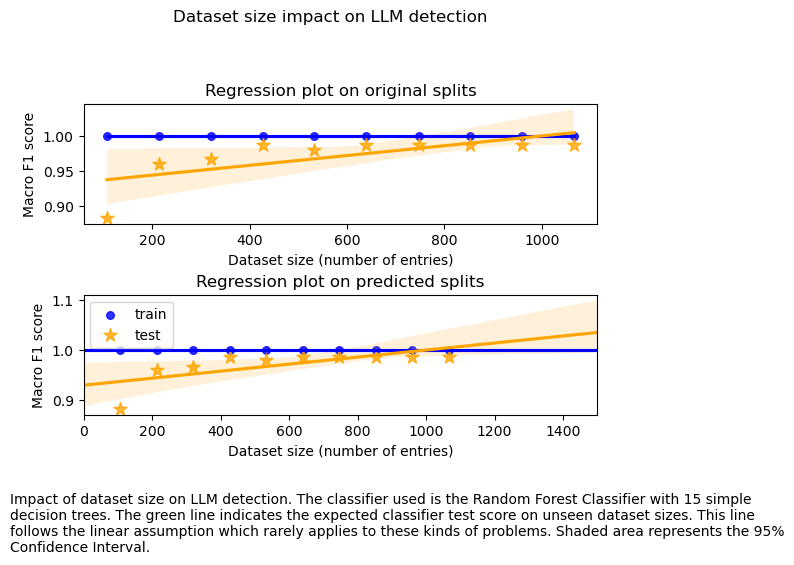
\includegraphics[width=14cm]{dataset_size.png}
		\centering
		\label{fig::dataset_size}
	\end{figure}
	
	\begin{figure}
		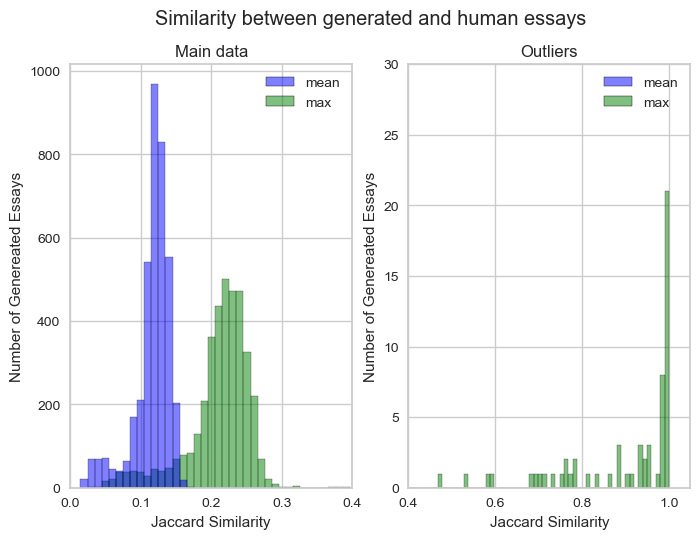
\includegraphics[width=14cm]{similarity.png}
		\centering
		\label{fig::similarity}
	\end{figure}
\end{document}